% !TEX encoding = UTF-8
% !TEX TS-program = pdflatex
% !TEX root = ../tesi.tex

%**************************************************************
\chapter{Analisi dei requisiti}
\label{cap:analisi-requisiti}

%**************************************************************

\section{Casi d'uso}
La progettazione dell'applicazione è iniziata con la stesura dei casi d'uso, supportati da diagrammi dei casi d'uso coerenti con lo standard UML.\\
I casi d'uso sono aumentati durante tutta la durata dello stage. Durante lo sviluppo, assieme al tutor, venivano individuate nuove funzionalità del programma per migliroare i risultati e aumentare l'automazione.

\begin{usecase}{0}{Scenario principale}
\usecaseactors{Utente}
\usecasepre{Il sistema è stato installato correttamente. L'utente ha aperto una \textit{shell} posizionata nella root dell'applicazione. (stato principale del sistema)}
\usecasedesc{Il sistema, tramite CLI (\textit{command line interface}), permette di:
    \begin{itemize}
        \item 1 inserire un file json;
        \item 2 inserire un file xmlsx;
        \item 3 personalizzare i parametri in output;
        \item 4 attivare o disattivare le funzionalità del programma;
        \item 5 creare una configurazione per il motore semantico di Engagent;
        \item 6 caricare automaticamente l'output in Engagent; 
        \item 7 inserire in input una configurazione già esistente
    \end{itemize}
}
\begin{figure}[H]
    \centering 
    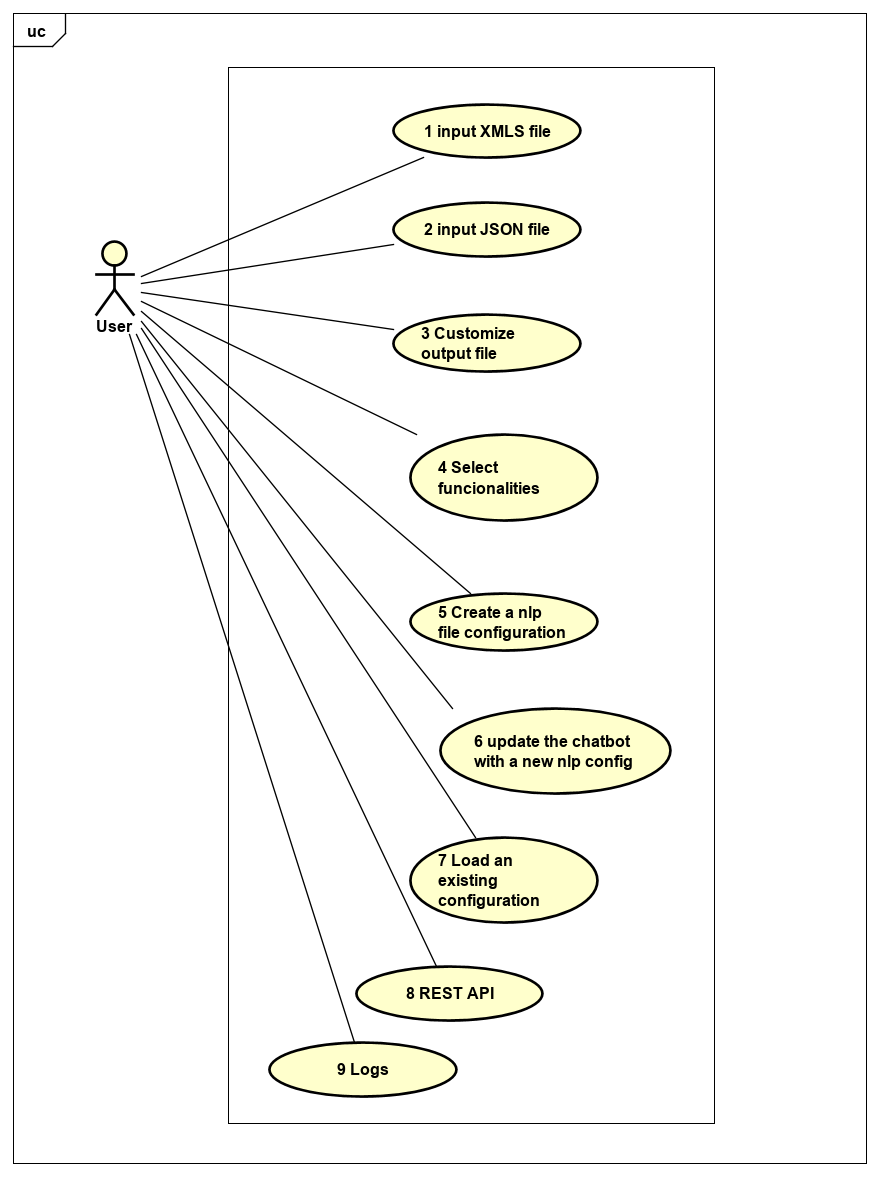
\includegraphics[width=0.9\columnwidth]{usecase/general_view.png} 
    \caption{Use Case - UC0: Scenario principale}
\end{figure}

\usecasepost{Il sistema è pronto per una nuova iterazione}
\label{uc:scenario-principale}
\end{usecase}

\begin{usecase}{1/2}{inserire un file json/xmlsx}
    \usecaseactors{Utente}
    \usecasepre{Il sistema mette a disposizione un comando per l'input di un file json/xmlsx}
    \usecasedesc{L'utente, tramite CLI, inserisce un file json/xmlsx}
    \usecasepost{Il sistema permette di inserire un nuovo file in input}
    \label{uc:1/2}
\end{usecase}

\begin{usecase}{3}{Personalizzazione parametri in output}
    \usecaseactors{Utente}
    \usecasepre{Il sistema mette a disposizione dei comandi per la personalizzazione dell'output}
    \usecasedesc{L'utente, tramite CLI, personalizza i parametri di output:
    \begin{itemize}
        \item 3.1 dominio;
        \item 3.2 lingua;
        \item 3.3 prefissi;
        \item 3.4 priorità delle regole.
    \end{itemize}
    }
    \usecasepost{Il sistema torna allo stato principale}
    \label{uc:3}
\end{usecase}

\begin{figure}[H]
    \centering 
    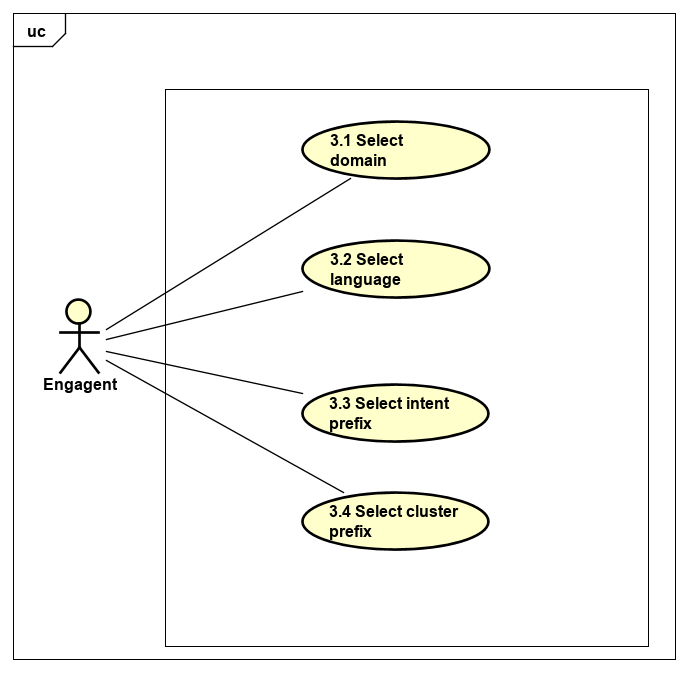
\includegraphics[width=0.9\columnwidth]{usecase/customize_output.png} 
    \caption{Use Case - UC3: Personalizzazione parametri in output}
\end{figure}

\begin{usecase}{3.1, 3.2, 3.3, 3.4}{Personalizzazione dominio/lingua/prefissi/priorità delle regole}
    \usecaseactors{Utente}
    \usecasepre{Il sistema mette a disposizione dei comandi per la personalizzazione dell'output}
    \usecasedesc{L'utente, tramite CLI, modifica il dominio/lingua/prefissi/priorità delle regole}
    \usecasepost{Il sistema permette di personalizzare nuovi parametri}
    \label{uc:3.1/3.2/3.3/3.4}
\end{usecase}

\begin{usecase}{4}{Attivare o disattivare le funzionalità del programma}
    \usecaseactors{Utente}
    \usecasepre{Il sistema mette a disposizione dei comandi per selezionare quali funzionalità del programma utilizzare}
    \usecasedesc{L'utente, tramite CLI, attiva o disattiva le seguenti funzionalità:
    \begin{itemize}
        \item 4.1 stemming sulle categorie;
        \item 4.2 validazione delle categorie attraverso le domande associate;
        \item 4.3 rimozione delle parole presenti in blacklist;
        \item 4.4 creazione di \textit{cluster};
        \item 4.5 creazione di \textit{intent}.
    \end{itemize}
    }
    \usecasepost{Il sistema torna allo stato principale}
    \label{uc:4}
\end{usecase}

\begin{usecase}{5}{Creare una configurazione compatibile con il motore semantico di Engagent}
    \usecaseactors{Utente}
    \usecasepre{Il sistema mette a disposizione un comando per la creazione della configurazione}
    \usecasedesc{L'utente, tramite CLI, crea una nuova configurazione}
    \usecasepost{\'E stato creato un nuovo file contenente la configurazione. Il sistema è tornato allo stato principale}
    \label{uc:5}
\end{usecase}
\begin{usecase}{6}{Caricare automaticamente la configurazione in Engagent}
    \usecaseactors{Utente}
    \usecasepre{Il sistema mette a disposizione un comando per caricare automaticamente il file contenente la configurare in Engagent}
    \usecasedesc{L'utente, tramite CLI, carica il file contenente la configurazione in Engagent}
    \usecasepost{Engagent contiene la nuova configurazione}
    \label{uc:6}
\end{usecase}
\begin{usecase}{7}{Inserire una configurazione già esistente}
    \usecaseactors{Utente}
    \usecasepre{Il sistema mette a disposizione un comando per l'input di una configurazione già esistente (vengono ereditate \textit{regole} e \textit{synset})}
    \usecasedesc{L'utente, tramite CLI, carica una configurazione esistente}
    \usecasepost{Il sistema contiene la configurazione di partenza}
    \label{uc:7}
\end{usecase}

\section{Tracciamento dei requisiti}

Da un'attenta analisi dei requisiti e degli use case effettuata sul progetto è stata stilata la tabella che traccia i requisiti in rapporto agli use case.\\
Il codice dei requisiti è così strutturato R[O/D][numero] dove:
\begin{enumerate}
	\item[R =] requisito
    \item[F =] funzionale
\end{enumerate}
\newpage

\begin{table}%
\caption{Tabella del tracciamento dei requisti funzionali}
\label{tab:requisiti-funzionali}
\begin{tabularx}{\textwidth}{lXl}
\hline\hline
\textbf{Requisito} & \textbf{Descrizione} & \textbf{Use Case}\\
\hline
RO-1     & L'utente può inserire un file Excel & UC1 \\
RO-2     & L'utente può inserire un file Json & UC2 \\
RO-3     & L'utente può personalizzare la configurazione & UC3 \\
RO-3.1   & L'utente può modificare il dominio della configurazione & UC3.1 \\
RO-3.2   & L'utente può modificare la lingua della configurazione & UC3.2 \\
RO-3.3   & L'utente può modificare i prefissi delle regole nella configurazione & UC 3.3\\
RO-3.4   & L'utente può modificare le priorità dei match nella configurazione & UC3.4 \\
RO-4     & L'utente può attivare o disattivare le funzionalità del programma & UC4 \\
RO-4.1   & L'utente può abilitare lo \glsfirstoccur{stemming} sulle categorie & UC4.1 \\
RO-4.2   & L'utente può disabilitare lo \glsfirstoccur{stemming} sulle categorie & UC4.1 \\
RO-4.3   & L'utente può abilitare la valdiazione delle categorie, attraverso le frasi associate& UC4.2 \\
RO-4.4   & L'utente può disabilitare la valdiazione delle categorie, attraverso le frasi associate & UC4.2 \\
RO-4.5   & L'utente può abilitare la creazione dei cluster & UC4.3 \\
RO-4.6   & L'utente può disabilitare la creazione dei cluster & UC4.4 \\
RO-4.7   & L'utente può abilitare la creazione degli intent& UC4.5 \\
RO-4.7   & L'utente può disabilitare la creazione degli intent& UC4.5 \\

\hline
\end{tabularx}
\end{table}%